\documentclass[1p]{elsarticle_modified}
%\bibliographystyle{elsarticle-num}

%\usepackage[colorlinks]{hyperref}
%\usepackage{abbrmath_seonhwa} %\Abb, \Ascr, \Acal ,\Abf, \Afrak
\usepackage{amsfonts}
\usepackage{amssymb}
\usepackage{amsmath}
\usepackage{amsthm}
\usepackage{scalefnt}
\usepackage{amsbsy}
\usepackage{kotex}
\usepackage{caption}
\usepackage{subfig}
\usepackage{color}
\usepackage{graphicx}
\usepackage{xcolor} %% white, black, red, green, blue, cyan, magenta, yellow
\usepackage{float}
\usepackage{setspace}
\usepackage{hyperref}

\usepackage{tikz}
\usetikzlibrary{arrows}

\usepackage{multirow}
\usepackage{array} % fixed length table
\usepackage{hhline}

%%%%%%%%%%%%%%%%%%%%%
\makeatletter
\renewcommand*\env@matrix[1][\arraystretch]{%
	\edef\arraystretch{#1}%
	\hskip -\arraycolsep
	\let\@ifnextchar\new@ifnextchar
	\array{*\c@MaxMatrixCols c}}
\makeatother %https://tex.stackexchange.com/questions/14071/how-can-i-increase-the-line-spacing-in-a-matrix
%%%%%%%%%%%%%%%

\usepackage[normalem]{ulem}

\newcommand{\msout}[1]{\ifmmode\text{\sout{\ensuremath{#1}}}\else\sout{#1}\fi}
%SOURCE: \msout is \stkout macro in https://tex.stackexchange.com/questions/20609/strikeout-in-math-mode

\newcommand{\cancel}[1]{
	\ifmmode
	{\color{red}\msout{#1}}
	\else
	{\color{red}\sout{#1}}
	\fi
}

\newcommand{\add}[1]{
	{\color{blue}\uwave{#1}}
}

\newcommand{\replace}[2]{
	\ifmmode
	{\color{red}\msout{#1}}{\color{blue}\uwave{#2}}
	\else
	{\color{red}\sout{#1}}{\color{blue}\uwave{#2}}
	\fi
}

\newcommand{\Sol}{\mathcal{S}} %segment
\newcommand{\D}{D} %diagram
\newcommand{\A}{\mathcal{A}} %arc


%%%%%%%%%%%%%%%%%%%%%%%%%%%%%5 test

\def\sl{\operatorname{\textup{SL}}(2,\Cbb)}
\def\psl{\operatorname{\textup{PSL}}(2,\Cbb)}
\def\quan{\mkern 1mu \triangleright \mkern 1mu}

\theoremstyle{definition}
\newtheorem{thm}{Theorem}[section]
\newtheorem{prop}[thm]{Proposition}
\newtheorem{lem}[thm]{Lemma}
\newtheorem{ques}[thm]{Question}
\newtheorem{cor}[thm]{Corollary}
\newtheorem{defn}[thm]{Definition}
\newtheorem{exam}[thm]{Example}
\newtheorem{rmk}[thm]{Remark}
\newtheorem{alg}[thm]{Algorithm}

\newcommand{\I}{\sqrt{-1}}
\begin{document}

%\begin{frontmatter}
%
%\title{Boundary parabolic representations of knots up to 8 crossings}
%
%%% Group authors per affiliation:
%\author{Yunhi Cho} 
%\address{Department of Mathematics, University of Seoul, Seoul, Korea}
%\ead{yhcho@uos.ac.kr}
%
%
%\author{Seonhwa Kim} %\fnref{s_kim}}
%\address{Center for Geometry and Physics, Institute for Basic Science, Pohang, 37673, Korea}
%\ead{ryeona17@ibs.re.kr}
%
%\author{Hyuk Kim}
%\address{Department of Mathematical Sciences, Seoul National University, Seoul 08826, Korea}
%\ead{hyukkim@snu.ac.kr}
%
%\author{Seokbeom Yoon}
%\address{Department of Mathematical Sciences, Seoul National University, Seoul, 08826,  Korea}
%\ead{sbyoon15@snu.ac.kr}
%
%\begin{abstract}
%We find all boundary parabolic representation of knots up to 8 crossings.
%
%\end{abstract}
%\begin{keyword}
%    \MSC[2010] 57M25 
%\end{keyword}
%
%\end{frontmatter}

%\linenumbers
%\tableofcontents
%
\newcommand\colored[1]{\textcolor{white}{\rule[-0.35ex]{0.8em}{1.4ex}}\kern-0.8em\color{red} #1}%
%\newcommand\colored[1]{\textcolor{white}{ #1}\kern-2.17ex	\textcolor{white}{ #1}\kern-1.81ex	\textcolor{white}{ #1}\kern-2.15ex\color{red}#1	}

{\Large $\underline{12a_{1144}~(K12a_{1144})}$}

\setlength{\tabcolsep}{10pt}
\renewcommand{\arraystretch}{1.6}
\vspace{1cm}\begin{tabular}{m{100pt}>{\centering\arraybackslash}m{274pt}}
\multirow{5}{120pt}{
	\centering
	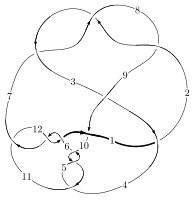
\includegraphics[width=112pt]{../../../GIT/diagram.site/Diagrams/png/1945_12a_1144.png}\\
\ \ \ A knot diagram\footnotemark}&
\allowdisplaybreaks
\textbf{Linearized knot diagam} \\
\cline{2-2}
 &
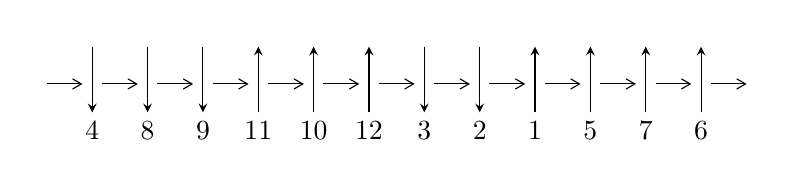
\begin{tikzpicture}[x=20pt, y=17pt]
	% nodes
	\node (C0) at (0, 0) {};
	\node (C1) at (1, 0) {};
	\node (C1U) at (1, +1) {};
	\node (C1D) at (1, -1) {4};

	\node (C2) at (2, 0) {};
	\node (C2U) at (2, +1) {};
	\node (C2D) at (2, -1) {8};

	\node (C3) at (3, 0) {};
	\node (C3U) at (3, +1) {};
	\node (C3D) at (3, -1) {9};

	\node (C4) at (4, 0) {};
	\node (C4U) at (4, +1) {};
	\node (C4D) at (4, -1) {11};

	\node (C5) at (5, 0) {};
	\node (C5U) at (5, +1) {};
	\node (C5D) at (5, -1) {10};

	\node (C6) at (6, 0) {};
	\node (C6U) at (6, +1) {};
	\node (C6D) at (6, -1) {12};

	\node (C7) at (7, 0) {};
	\node (C7U) at (7, +1) {};
	\node (C7D) at (7, -1) {3};

	\node (C8) at (8, 0) {};
	\node (C8U) at (8, +1) {};
	\node (C8D) at (8, -1) {2};

	\node (C9) at (9, 0) {};
	\node (C9U) at (9, +1) {};
	\node (C9D) at (9, -1) {1};

	\node (C10) at (10, 0) {};
	\node (C10U) at (10, +1) {};
	\node (C10D) at (10, -1) {5};

	\node (C11) at (11, 0) {};
	\node (C11U) at (11, +1) {};
	\node (C11D) at (11, -1) {7};

	\node (C12) at (12, 0) {};
	\node (C12U) at (12, +1) {};
	\node (C12D) at (12, -1) {6};
	\node (C13) at (13, 0) {};

	% arrows
	\draw[->,>={angle 60}]
	(C0) edge (C1) (C1) edge (C2) (C2) edge (C3) (C3) edge (C4) (C4) edge (C5) (C5) edge (C6) (C6) edge (C7) (C7) edge (C8) (C8) edge (C9) (C9) edge (C10) (C10) edge (C11) (C11) edge (C12) (C12) edge (C13) ;	\draw[->,>=stealth]
	(C1U) edge (C1D) (C2U) edge (C2D) (C3U) edge (C3D) (C4D) edge (C4U) (C5D) edge (C5U) (C6D) edge (C6U) (C7U) edge (C7D) (C8U) edge (C8D) (C9D) edge (C9U) (C10D) edge (C10U) (C11D) edge (C11U) (C12D) edge (C12U) ;
	\end{tikzpicture} \\
\hhline{~~} \\& 
\textbf{Solving Sequence} \\ \cline{2-2} 
 &
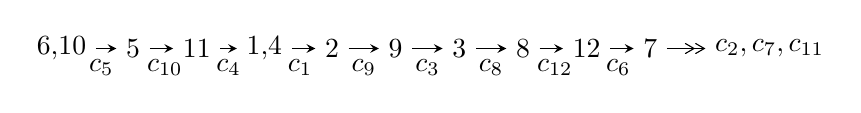
\begin{tikzpicture}[x=23pt, y=7pt]
	% node
	\node (A0) at (-1/8, 0) {6,10};
	\node (A1) at (1, 0) {5};
	\node (A2) at (2, 0) {11};
	\node (A3) at (49/16, 0) {1,4};
	\node (A4) at (33/8, 0) {2};
	\node (A5) at (41/8, 0) {9};
	\node (A6) at (49/8, 0) {3};
	\node (A7) at (57/8, 0) {8};
	\node (A8) at (65/8, 0) {12};
	\node (A9) at (73/8, 0) {7};
	\node (C1) at (1/2, -1) {$c_{5}$};
	\node (C2) at (3/2, -1) {$c_{10}$};
	\node (C3) at (5/2, -1) {$c_{4}$};
	\node (C4) at (29/8, -1) {$c_{1}$};
	\node (C5) at (37/8, -1) {$c_{9}$};
	\node (C6) at (45/8, -1) {$c_{3}$};
	\node (C7) at (53/8, -1) {$c_{8}$};
	\node (C8) at (61/8, -1) {$c_{12}$};
	\node (C9) at (69/8, -1) {$c_{6}$};
	\node (A10) at (11, 0) {$c_{2},c_{7},c_{11}$};

	% edge
	\draw[->,>=stealth]	
	(A0) edge (A1) (A1) edge (A2) (A2) edge (A3) (A3) edge (A4) (A4) edge (A5) (A5) edge (A6) (A6) edge (A7) (A7) edge (A8) (A8) edge (A9) ;
	\draw[->>,>={angle 60}]	
	(A9) edge (A10);
\end{tikzpicture} \\ 

\end{tabular} \\

\footnotetext{
The image of knot diagram is generated by the software ``\textbf{Draw programme}" developed by Andrew Bartholomew(\url{http://www.layer8.co.uk/maths/draw/index.htm\#Running-draw}), where we modified some parts for our purpose(\url{https://github.com/CATsTAILs/LinksPainter}).
}\phantom \\ \newline 
\centering \textbf{Ideals for irreducible components\footnotemark of $X_{\text{par}}$} 
 
\begin{align*}
I^u_{1}&=\langle 
b- u,\;- u^{31}+u^{30}+\cdots+32 a+1,\;u^{32}+20 u^{30}+\cdots+2 u+1\rangle \\
I^u_{2}&=\langle 
-5.88169\times10^{23} u^{41}+2.40634\times10^{24} u^{40}+\cdots+2.85857\times10^{25} b-1.53616\times10^{25},\\
\phantom{I^u_{2}}&\phantom{= \langle  }-2.91738\times10^{25} u^{41}+3.09920\times10^{25} u^{40}+\cdots+2.85857\times10^{25} a+4.18097\times10^{25},\;u^{42}- u^{41}+\cdots-2 u+1\rangle \\
I^u_{3}&=\langle 
b+u,\;a^5- a^4+2 a^3- a^2+a-1,\;u^2+1\rangle \\
\\
\end{align*}
\raggedright * 3 irreducible components of $\dim_{\mathbb{C}}=0$, with total 84 representations.\\
\footnotetext{All coefficients of polynomials are rational numbers. But the coefficients are sometimes approximated in decimal forms when there is not enough margin.}
\newpage
\renewcommand{\arraystretch}{1}
\centering \section*{I. $I^u_{1}= \langle b- u,\;- u^{31}+u^{30}+\cdots+32 a+1,\;u^{32}+20 u^{30}+\cdots+2 u+1 \rangle$}
\flushleft \textbf{(i) Arc colorings}\\
\begin{tabular}{m{7pt} m{180pt} m{7pt} m{180pt} }
\flushright $a_{6}=$&$\begin{pmatrix}1\\0\end{pmatrix}$ \\
\flushright $a_{10}=$&$\begin{pmatrix}0\\u\end{pmatrix}$ \\
\flushright $a_{5}=$&$\begin{pmatrix}1\\u^2\end{pmatrix}$ \\
\flushright $a_{11}=$&$\begin{pmatrix}u\\u^3+u\end{pmatrix}$ \\
\flushright $a_{1}=$&$\begin{pmatrix}0.0312500 u^{31}-0.0312500 u^{30}+\cdots+2.96875 u-0.0312500\\u\end{pmatrix}$ \\
\flushright $a_{4}=$&$\begin{pmatrix}u^2+1\\u^4+2 u^2\end{pmatrix}$ \\
\flushright $a_{2}=$&$\begin{pmatrix}0.0312500 u^{31}-0.0312500 u^{30}+\cdots+1.96875 u-0.0312500\\0.0312500 u^{31}-0.0312500 u^{30}+\cdots+0.968750 u-0.0312500\end{pmatrix}$ \\
\flushright $a_{9}=$&$\begin{pmatrix}0.0312500 u^{31}-0.0312500 u^{30}+\cdots-0.0937500 u-0.0937500\\0.0312500 u^{31}-0.0312500 u^{30}+\cdots+0.968750 u-0.0312500\end{pmatrix}$ \\
\flushright $a_{3}=$&$\begin{pmatrix}\frac{9}{16} u^{31}-\frac{1}{4} u^{30}+\cdots+\frac{9}{4} u+\frac{21}{16}\\\frac{3}{8} u^{31}+\frac{1}{4} u^{30}+\cdots+\frac{19}{16} u+\frac{5}{16}\end{pmatrix}$ \\
\flushright $a_{8}=$&$\begin{pmatrix}-\frac{1}{16} u^{31}-\frac{1}{16} u^{30}+\cdots-\frac{7}{8} u-\frac{5}{8}\\\frac{1}{8} u^{31}-\frac{7}{16} u^{30}+\cdots-\frac{1}{2} u-\frac{17}{16}\end{pmatrix}$ \\
\flushright $a_{12}=$&$\begin{pmatrix}0.0312500 u^{31}-0.0312500 u^{30}+\cdots+1.96875 u-0.0312500\\u\end{pmatrix}$ \\
\flushright $a_{7}=$&$\begin{pmatrix}0.0312500 u^{31}+0.0312500 u^{30}+\cdots+0.0937500 u+1.03125\\- u^2\end{pmatrix}$\\&\end{tabular}
\flushleft \textbf{(ii) Obstruction class $= -1$}\\~\\
\flushleft \textbf{(iii) Cusp Shapes $= \frac{11}{8} u^{31}-\frac{1}{8} u^{30}+\cdots+8 u+\frac{7}{2}$}\\~\\
\newpage\renewcommand{\arraystretch}{1}
\flushleft \textbf{(iv) u-Polynomials at the component}\newline \\
\begin{tabular}{m{50pt}|m{274pt}}
Crossings & \hspace{64pt}u-Polynomials at each crossing \\
\hline $$\begin{aligned}c_{1}\end{aligned}$$&$\begin{aligned}
&u^{32}-7 u^{31}+\cdots-629 u+136
\end{aligned}$\\
\hline $$\begin{aligned}c_{2},c_{7},c_{8}\end{aligned}$$&$\begin{aligned}
&u^{32}-3 u^{31}+\cdots-9 u+2
\end{aligned}$\\
\hline $$\begin{aligned}c_{3}\end{aligned}$$&$\begin{aligned}
&u^{32}+3 u^{31}+\cdots-45 u+10
\end{aligned}$\\
\hline $$\begin{aligned}c_{4},c_{5},c_{6}\\c_{10},c_{11},c_{12}\end{aligned}$$&$\begin{aligned}
&u^{32}+20 u^{30}+\cdots-2 u+1
\end{aligned}$\\
\hline $$\begin{aligned}c_{9}\end{aligned}$$&$\begin{aligned}
&u^{32}-21 u^{31}+\cdots-31521 u+3794
\end{aligned}$\\
\hline
\end{tabular}\\~\\
\newpage\renewcommand{\arraystretch}{1}
\flushleft \textbf{(v) Riley Polynomials at the component}\newline \\
\begin{tabular}{m{50pt}|m{274pt}}
Crossings & \hspace{64pt}Riley Polynomials at each crossing \\
\hline $$\begin{aligned}c_{1}\end{aligned}$$&$\begin{aligned}
&y^{32}+9 y^{31}+\cdots+185079 y+18496
\end{aligned}$\\
\hline $$\begin{aligned}c_{2},c_{7},c_{8}\end{aligned}$$&$\begin{aligned}
&y^{32}+29 y^{31}+\cdots+3 y+4
\end{aligned}$\\
\hline $$\begin{aligned}c_{3}\end{aligned}$$&$\begin{aligned}
&y^{32}+y^{31}+\cdots+1795 y+100
\end{aligned}$\\
\hline $$\begin{aligned}c_{4},c_{5},c_{6}\\c_{10},c_{11},c_{12}\end{aligned}$$&$\begin{aligned}
&y^{32}+40 y^{31}+\cdots+10 y+1
\end{aligned}$\\
\hline $$\begin{aligned}c_{9}\end{aligned}$$&$\begin{aligned}
&y^{32}+9 y^{31}+\cdots+46718595 y+14394436
\end{aligned}$\\
\hline
\end{tabular}\\~\\
\newpage\flushleft \textbf{(vi) Complex Volumes and Cusp Shapes}
$$\begin{array}{c|c|c}  
\text{Solutions to }I^u_{1}& \I (\text{vol} + \sqrt{-1}CS) & \text{Cusp shape}\\
 \hline 
\begin{aligned}
u &= -0.606629 + 0.369922 I \\
a &= -1.66986 + 0.58326 I \\
b &= -0.606629 + 0.369922 I\end{aligned}
 & \phantom{-}5.08010 - 7.21382 I & \phantom{-}6.51491 + 8.36258 I \\ \hline\begin{aligned}
u &= -0.606629 - 0.369922 I \\
a &= -1.66986 - 0.58326 I \\
b &= -0.606629 - 0.369922 I\end{aligned}
 & \phantom{-}5.08010 + 7.21382 I & \phantom{-}6.51491 - 8.36258 I \\ \hline\begin{aligned}
u &= \phantom{-}0.629670 + 0.175324 I \\
a &= \phantom{-}1.56872 + 0.28026 I \\
b &= \phantom{-}0.629670 + 0.175324 I\end{aligned}
 & \phantom{-}6.58025 - 1.12952 I & \phantom{-}10.00433 - 1.13663 I \\ \hline\begin{aligned}
u &= \phantom{-}0.629670 - 0.175324 I \\
a &= \phantom{-}1.56872 - 0.28026 I \\
b &= \phantom{-}0.629670 - 0.175324 I\end{aligned}
 & \phantom{-}6.58025 + 1.12952 I & \phantom{-}10.00433 + 1.13663 I \\ \hline\begin{aligned}
u &= \phantom{-}0.546847 + 0.354433 I \\
a &= \phantom{-}1.56713 + 0.62149 I \\
b &= \phantom{-}0.546847 + 0.354433 I\end{aligned}
 & -0.24655 + 3.89301 I & \phantom{-}1.84831 - 8.81175 I \\ \hline\begin{aligned}
u &= \phantom{-}0.546847 - 0.354433 I \\
a &= \phantom{-}1.56713 - 0.62149 I \\
b &= \phantom{-}0.546847 - 0.354433 I\end{aligned}
 & -0.24655 - 3.89301 I & \phantom{-}1.84831 + 8.81175 I \\ \hline\begin{aligned}
u &= -0.046705 + 1.401200 I \\
a &= -0.34108 - 1.47427 I \\
b &= -0.046705 + 1.401200 I\end{aligned}
 & -0.35213 - 5.09138 I & -0.46090 + 3.41418 I \\ \hline\begin{aligned}
u &= -0.046705 - 1.401200 I \\
a &= -0.34108 + 1.47427 I \\
b &= -0.046705 - 1.401200 I\end{aligned}
 & -0.35213 + 5.09138 I & -0.46090 - 3.41418 I \\ \hline\begin{aligned}
u &= \phantom{-}0.02438 + 1.43670 I \\
a &= \phantom{-}0.155902 - 1.256460 I \\
b &= \phantom{-}0.02438 + 1.43670 I\end{aligned}
 & -6.57448 + 2.07353 I & -3.81450 - 3.36266 I \\ \hline\begin{aligned}
u &= \phantom{-}0.02438 - 1.43670 I \\
a &= \phantom{-}0.155902 + 1.256460 I \\
b &= \phantom{-}0.02438 - 1.43670 I\end{aligned}
 & -6.57448 - 2.07353 I & -3.81450 + 3.36266 I\\
 \hline 
 \end{array}$$\newpage$$\begin{array}{c|c|c}  
\text{Solutions to }I^u_{1}& \I (\text{vol} + \sqrt{-1}CS) & \text{Cusp shape}\\
 \hline 
\begin{aligned}
u &= -0.353670 + 0.399081 I \\
a &= -1.25094 + 0.96324 I \\
b &= -0.353670 + 0.399081 I\end{aligned}
 & \phantom{-}1.33414 - 1.26458 I & \phantom{-}2.44160 + 5.52381 I \\ \hline\begin{aligned}
u &= -0.353670 - 0.399081 I \\
a &= -1.25094 - 0.96324 I \\
b &= -0.353670 - 0.399081 I\end{aligned}
 & \phantom{-}1.33414 + 1.26458 I & \phantom{-}2.44160 - 5.52381 I \\ \hline\begin{aligned}
u &= -0.103781 + 0.515513 I \\
a &= -0.57149 + 1.83224 I \\
b &= -0.103781 + 0.515513 I\end{aligned}
 & \phantom{-}4.24971 + 4.08144 I & \phantom{-}5.01801 - 1.73350 I \\ \hline\begin{aligned}
u &= -0.103781 - 0.515513 I \\
a &= -0.57149 - 1.83224 I \\
b &= -0.103781 - 0.515513 I\end{aligned}
 & \phantom{-}4.24971 - 4.08144 I & \phantom{-}5.01801 + 1.73350 I \\ \hline\begin{aligned}
u &= -0.477770 + 0.219464 I \\
a &= -1.326770 + 0.440538 I \\
b &= -0.477770 + 0.219464 I\end{aligned}
 & \phantom{-}0.940582 - 0.674762 I & \phantom{-}6.97731 + 2.54975 I \\ \hline\begin{aligned}
u &= -0.477770 - 0.219464 I \\
a &= -1.326770 - 0.440538 I \\
b &= -0.477770 - 0.219464 I\end{aligned}
 & \phantom{-}0.940582 + 0.674762 I & \phantom{-}6.97731 - 2.54975 I \\ \hline\begin{aligned}
u &= -0.26977 + 1.48889 I \\
a &= -1.178040 - 0.476261 I \\
b &= -0.26977 + 1.48889 I\end{aligned}
 & -4.22469 - 5.46260 I & \phantom{-0.000000 } 0 \\ \hline\begin{aligned}
u &= -0.26977 - 1.48889 I \\
a &= -1.178040 + 0.476261 I \\
b &= -0.26977 - 1.48889 I\end{aligned}
 & -4.22469 + 5.46260 I & \phantom{-0.000000 } 0 \\ \hline\begin{aligned}
u &= \phantom{-}0.146914 + 0.429589 I \\
a &= \phantom{-}0.64149 + 1.38146 I \\
b &= \phantom{-}0.146914 + 0.429589 I\end{aligned}
 & -0.98864 - 1.13789 I & -1.40453 + 1.40100 I \\ \hline\begin{aligned}
u &= \phantom{-}0.146914 - 0.429589 I \\
a &= \phantom{-}0.64149 - 1.38146 I \\
b &= \phantom{-}0.146914 - 0.429589 I\end{aligned}
 & -0.98864 + 1.13789 I & -1.40453 - 1.40100 I\\
 \hline 
 \end{array}$$\newpage$$\begin{array}{c|c|c}  
\text{Solutions to }I^u_{1}& \I (\text{vol} + \sqrt{-1}CS) & \text{Cusp shape}\\
 \hline 
\begin{aligned}
u &= \phantom{-}0.28852 + 1.54432 I \\
a &= \phantom{-}1.092720 - 0.277920 I \\
b &= \phantom{-}0.28852 + 1.54432 I\end{aligned}
 & -11.21850 + 6.79287 I & \phantom{-0.000000 } 0 \\ \hline\begin{aligned}
u &= \phantom{-}0.28852 - 1.54432 I \\
a &= \phantom{-}1.092720 + 0.277920 I \\
b &= \phantom{-}0.28852 - 1.54432 I\end{aligned}
 & -11.21850 - 6.79287 I & \phantom{-0.000000 } 0 \\ \hline\begin{aligned}
u &= \phantom{-}0.34148 + 1.53474 I \\
a &= \phantom{-}1.241970 - 0.181115 I \\
b &= \phantom{-}0.34148 + 1.53474 I\end{aligned}
 & -7.3512 + 14.7885 I & \phantom{-0.000000 } 0 \\ \hline\begin{aligned}
u &= \phantom{-}0.34148 - 1.53474 I \\
a &= \phantom{-}1.241970 + 0.181115 I \\
b &= \phantom{-}0.34148 - 1.53474 I\end{aligned}
 & -7.3512 - 14.7885 I & \phantom{-0.000000 } 0 \\ \hline\begin{aligned}
u &= -0.32266 + 1.54438 I \\
a &= -1.177440 - 0.201810 I \\
b &= -0.32266 + 1.54438 I\end{aligned}
 & -12.7964 - 10.9677 I & \phantom{-0.000000 } 0 \\ \hline\begin{aligned}
u &= -0.32266 - 1.54438 I \\
a &= -1.177440 + 0.201810 I \\
b &= -0.32266 - 1.54438 I\end{aligned}
 & -12.7964 + 10.9677 I & \phantom{-0.000000 } 0 \\ \hline\begin{aligned}
u &= \phantom{-}0.24178 + 1.58208 I \\
a &= \phantom{-}0.886317 - 0.267032 I \\
b &= \phantom{-}0.24178 + 1.58208 I\end{aligned}
 & -11.98810 + 6.51283 I & \phantom{-0.000000 } 0 \\ \hline\begin{aligned}
u &= \phantom{-}0.24178 - 1.58208 I \\
a &= \phantom{-}0.886317 + 0.267032 I \\
b &= \phantom{-}0.24178 - 1.58208 I\end{aligned}
 & -11.98810 - 6.51283 I & \phantom{-0.000000 } 0 \\ \hline\begin{aligned}
u &= -0.19813 + 1.59690 I \\
a &= -0.728237 - 0.294996 I \\
b &= -0.19813 + 1.59690 I\end{aligned}
 & -14.7686 - 2.5621 I & \phantom{-0.000000 } 0 \\ \hline\begin{aligned}
u &= -0.19813 - 1.59690 I \\
a &= -0.728237 + 0.294996 I \\
b &= -0.19813 - 1.59690 I\end{aligned}
 & -14.7686 + 2.5621 I & \phantom{-0.000000 } 0\\
 \hline 
 \end{array}$$\newpage$$\begin{array}{c|c|c}  
\text{Solutions to }I^u_{1}& \I (\text{vol} + \sqrt{-1}CS) & \text{Cusp shape}\\
 \hline 
\begin{aligned}
u &= \phantom{-}0.15953 + 1.60567 I \\
a &= \phantom{-}0.589601 - 0.320624 I \\
b &= \phantom{-}0.15953 + 1.60567 I\end{aligned}
 & -10.18300 - 1.30058 I & \phantom{-0.000000 } 0 \\ \hline\begin{aligned}
u &= \phantom{-}0.15953 - 1.60567 I \\
a &= \phantom{-}0.589601 + 0.320624 I \\
b &= \phantom{-}0.15953 - 1.60567 I\end{aligned}
 & -10.18300 + 1.30058 I & \phantom{-0.000000 } 0\\
 \hline 
 \end{array}$$\newpage\newpage\renewcommand{\arraystretch}{1}
\centering \section*{II. $I^u_{2}= \langle -5.88\times10^{23} u^{41}+2.41\times10^{24} u^{40}+\cdots+2.86\times10^{25} b-1.54\times10^{25},\;-2.92\times10^{25} u^{41}+3.10\times10^{25} u^{40}+\cdots+2.86\times10^{25} a+4.18\times10^{25},\;u^{42}- u^{41}+\cdots-2 u+1 \rangle$}
\flushleft \textbf{(i) Arc colorings}\\
\begin{tabular}{m{7pt} m{180pt} m{7pt} m{180pt} }
\flushright $a_{6}=$&$\begin{pmatrix}1\\0\end{pmatrix}$ \\
\flushright $a_{10}=$&$\begin{pmatrix}0\\u\end{pmatrix}$ \\
\flushright $a_{5}=$&$\begin{pmatrix}1\\u^2\end{pmatrix}$ \\
\flushright $a_{11}=$&$\begin{pmatrix}u\\u^3+u\end{pmatrix}$ \\
\flushright $a_{1}=$&$\begin{pmatrix}1.02058 u^{41}-1.08418 u^{40}+\cdots-17.0532 u-1.46261\\0.0205757 u^{41}-0.0841800 u^{40}+\cdots-3.05321 u+0.537389\end{pmatrix}$ \\
\flushright $a_{4}=$&$\begin{pmatrix}u^2+1\\u^4+2 u^2\end{pmatrix}$ \\
\flushright $a_{2}=$&$\begin{pmatrix}0.982739 u^{41}-0.799526 u^{40}+\cdots-16.2270 u-1.88182\\0.0674687 u^{41}-0.121292 u^{40}+\cdots-2.75800 u+0.420716\end{pmatrix}$ \\
\flushright $a_{9}=$&$\begin{pmatrix}1.03523 u^{41}-1.08688 u^{40}+\cdots-19.2542 u-0.861618\\0.0146583 u^{41}-0.00269680 u^{40}+\cdots-1.20099 u+0.600993\end{pmatrix}$ \\
\flushright $a_{3}=$&$\begin{pmatrix}0.0215507 u^{41}+0.0984422 u^{40}+\cdots-16.5835 u+5.10219\\0.359884 u^{41}-0.273709 u^{40}+\cdots-2.93547 u+1.06141\end{pmatrix}$ \\
\flushright $a_{8}=$&$\begin{pmatrix}1.19912 u^{41}-1.61059 u^{40}+\cdots-21.6738 u+1.42196\\0.150022 u^{41}-0.407409 u^{40}+\cdots+3.68385 u+0.0765627\end{pmatrix}$ \\
\flushright $a_{12}=$&$\begin{pmatrix}u^{41}- u^{40}+\cdots-14 u-2\\0.0205757 u^{41}-0.0841800 u^{40}+\cdots-3.05321 u+0.537389\end{pmatrix}$ \\
\flushright $a_{7}=$&$\begin{pmatrix}-0.537389 u^{41}+0.557965 u^{40}+\cdots-10.9961 u-0.978429\\-0.0636043 u^{41}+0.0576870 u^{40}+\cdots+0.578540 u+0.979424\end{pmatrix}$\\&\end{tabular}
\flushleft \textbf{(ii) Obstruction class $= -1$}\\~\\
\flushleft \textbf{(iii) Cusp Shapes $= -\frac{72222077540047874114658048}{28585672337950454401808201} u^{41}+\frac{29500521900029629423443720}{28585672337950454401808201} u^{40}+\cdots-\frac{299812736301611137792225292}{28585672337950454401808201} u+\frac{106417593374116830733331718}{28585672337950454401808201}$}\\~\\
\newpage\renewcommand{\arraystretch}{1}
\flushleft \textbf{(iv) u-Polynomials at the component}\newline \\
\begin{tabular}{m{50pt}|m{274pt}}
Crossings & \hspace{64pt}u-Polynomials at each crossing \\
\hline $$\begin{aligned}c_{1}\end{aligned}$$&$\begin{aligned}
&(u^{21}-5 u^{20}+\cdots-11 u+3)^{2}
\end{aligned}$\\
\hline $$\begin{aligned}c_{2},c_{7},c_{8}\end{aligned}$$&$\begin{aligned}
&(u^{21}+u^{20}+\cdots- u-1)^{2}
\end{aligned}$\\
\hline $$\begin{aligned}c_{3}\end{aligned}$$&$\begin{aligned}
&(u^{21}- u^{20}+\cdots-3 u-1)^{2}
\end{aligned}$\\
\hline $$\begin{aligned}c_{4},c_{5},c_{6}\\c_{10},c_{11},c_{12}\end{aligned}$$&$\begin{aligned}
&u^{42}+u^{41}+\cdots+2 u+1
\end{aligned}$\\
\hline $$\begin{aligned}c_{9}\end{aligned}$$&$\begin{aligned}
&(u^{21}+7 u^{20}+\cdots+3 u-1)^{2}
\end{aligned}$\\
\hline
\end{tabular}\\~\\
\newpage\renewcommand{\arraystretch}{1}
\flushleft \textbf{(v) Riley Polynomials at the component}\newline \\
\begin{tabular}{m{50pt}|m{274pt}}
Crossings & \hspace{64pt}Riley Polynomials at each crossing \\
\hline $$\begin{aligned}c_{1}\end{aligned}$$&$\begin{aligned}
&(y^{21}+3 y^{20}+\cdots-41 y-9)^{2}
\end{aligned}$\\
\hline $$\begin{aligned}c_{2},c_{7},c_{8}\end{aligned}$$&$\begin{aligned}
&(y^{21}+19 y^{20}+\cdots+3 y-1)^{2}
\end{aligned}$\\
\hline $$\begin{aligned}c_{3}\end{aligned}$$&$\begin{aligned}
&(y^{21}- y^{20}+\cdots+3 y-1)^{2}
\end{aligned}$\\
\hline $$\begin{aligned}c_{4},c_{5},c_{6}\\c_{10},c_{11},c_{12}\end{aligned}$$&$\begin{aligned}
&y^{42}+35 y^{41}+\cdots-32 y+1
\end{aligned}$\\
\hline $$\begin{aligned}c_{9}\end{aligned}$$&$\begin{aligned}
&(y^{21}+15 y^{20}+\cdots+27 y-1)^{2}
\end{aligned}$\\
\hline
\end{tabular}\\~\\
\newpage\flushleft \textbf{(vi) Complex Volumes and Cusp Shapes}
$$\begin{array}{c|c|c}  
\text{Solutions to }I^u_{2}& \I (\text{vol} + \sqrt{-1}CS) & \text{Cusp shape}\\
 \hline 
\begin{aligned}
u &= \phantom{-}0.142789 + 0.981947 I \\
a &= -0.400579 + 1.077330 I \\
b &= -0.255559 + 0.080028 I\end{aligned}
 & \phantom{-}4.29768 + 4.29720 I & \phantom{-}6.75143 - 3.93304 I \\ \hline\begin{aligned}
u &= \phantom{-}0.142789 - 0.981947 I \\
a &= -0.400579 - 1.077330 I \\
b &= -0.255559 - 0.080028 I\end{aligned}
 & \phantom{-}4.29768 - 4.29720 I & \phantom{-}6.75143 + 3.93304 I \\ \hline\begin{aligned}
u &= \phantom{-}0.803564 + 0.620127 I \\
a &= -0.854334 - 0.849675 I \\
b &= -0.07438 - 1.45158 I\end{aligned}
 & -4.65974 + 2.68588 I & -1.85070 - 3.67518 I \\ \hline\begin{aligned}
u &= \phantom{-}0.803564 - 0.620127 I \\
a &= -0.854334 + 0.849675 I \\
b &= -0.07438 + 1.45158 I\end{aligned}
 & -4.65974 - 2.68588 I & -1.85070 + 3.67518 I \\ \hline\begin{aligned}
u &= -0.892757 + 0.485854 I \\
a &= \phantom{-}1.04420 - 0.99396 I \\
b &= \phantom{-}0.18002 - 1.46427 I\end{aligned}
 & -6.19421 - 6.51836 I & -3.49661 + 6.69162 I \\ \hline\begin{aligned}
u &= -0.892757 - 0.485854 I \\
a &= \phantom{-}1.04420 + 0.99396 I \\
b &= \phantom{-}0.18002 + 1.46427 I\end{aligned}
 & -6.19421 + 6.51836 I & -3.49661 - 6.69162 I \\ \hline\begin{aligned}
u &= \phantom{-}0.816854 + 0.532908 I \\
a &= -0.987760 - 0.874778 I \\
b &= -0.12904 - 1.43500 I\end{aligned}
 & -4.44976 + 2.73152 I & -0.80842 - 2.00184 I \\ \hline\begin{aligned}
u &= \phantom{-}0.816854 - 0.532908 I \\
a &= -0.987760 + 0.874778 I \\
b &= -0.12904 + 1.43500 I\end{aligned}
 & -4.44976 - 2.73152 I & -0.80842 + 2.00184 I \\ \hline\begin{aligned}
u &= \phantom{-}0.920413 + 0.451372 I \\
a &= -1.08540 - 1.03931 I \\
b &= -0.20956 - 1.46882 I\end{aligned}
 & -0.91901 + 10.18330 I & \phantom{-}1.25382 - 7.21296 I \\ \hline\begin{aligned}
u &= \phantom{-}0.920413 - 0.451372 I \\
a &= -1.08540 + 1.03931 I \\
b &= -0.20956 + 1.46882 I\end{aligned}
 & -0.91901 - 10.18330 I & \phantom{-}1.25382 + 7.21296 I\\
 \hline 
 \end{array}$$\newpage$$\begin{array}{c|c|c}  
\text{Solutions to }I^u_{2}& \I (\text{vol} + \sqrt{-1}CS) & \text{Cusp shape}\\
 \hline 
\begin{aligned}
u &= -0.769634 + 0.726428 I \\
a &= \phantom{-}0.688478 - 0.808047 I \\
b &= \phantom{-}0.00133 - 1.45662 I\end{aligned}
 & -6.94955 + 0.90110 I & -5.44354 - 1.25880 I \\ \hline\begin{aligned}
u &= -0.769634 - 0.726428 I \\
a &= \phantom{-}0.688478 + 0.808047 I \\
b &= \phantom{-}0.00133 + 1.45662 I\end{aligned}
 & -6.94955 - 0.90110 I & -5.44354 + 1.25880 I \\ \hline\begin{aligned}
u &= -0.405760 + 0.979630 I \\
a &= \phantom{-}0.166067 - 0.368101 I \\
b &= -0.194828 - 1.239410 I\end{aligned}
 & \phantom{-}0.10785 - 2.26276 I & -0.12423 + 3.11409 I \\ \hline\begin{aligned}
u &= -0.405760 - 0.979630 I \\
a &= \phantom{-}0.166067 + 0.368101 I \\
b &= -0.194828 + 1.239410 I\end{aligned}
 & \phantom{-}0.10785 + 2.26276 I & -0.12423 - 3.11409 I \\ \hline\begin{aligned}
u &= -0.064971 + 1.059860 I \\
a &= \phantom{-}0.213265 + 0.829397 I \\
b &= \phantom{-}0.155643 - 0.110588 I\end{aligned}
 & -1.26832 - 1.59690 I & \phantom{-}3.13274 + 4.73829 I \\ \hline\begin{aligned}
u &= -0.064971 - 1.059860 I \\
a &= \phantom{-}0.213265 - 0.829397 I \\
b &= \phantom{-}0.155643 + 0.110588 I\end{aligned}
 & -1.26832 + 1.59690 I & \phantom{-}3.13274 - 4.73829 I \\ \hline\begin{aligned}
u &= \phantom{-}0.211058 + 1.064720 I \\
a &= \phantom{-}0.031919 - 0.161023 I \\
b &= \phantom{-}0.211058 - 1.064720 I\end{aligned}
 & -4.11368\phantom{ +0.000000I} & -8.21539 + 0. I\phantom{ +0.000000I} \\ \hline\begin{aligned}
u &= \phantom{-}0.211058 - 1.064720 I \\
a &= \phantom{-}0.031919 + 0.161023 I \\
b &= \phantom{-}0.211058 + 1.064720 I\end{aligned}
 & -4.11368\phantom{ +0.000000I} & -8.21539 + 0. I\phantom{ +0.000000I} \\ \hline\begin{aligned}
u &= \phantom{-}0.758158 + 0.793503 I \\
a &= -0.585546 - 0.804617 I \\
b &= \phantom{-}0.04392 - 1.46343 I\end{aligned}
 & -1.96895 - 4.48385 I & -0.56586 + 2.47352 I \\ \hline\begin{aligned}
u &= \phantom{-}0.758158 - 0.793503 I \\
a &= -0.585546 + 0.804617 I \\
b &= \phantom{-}0.04392 + 1.46343 I\end{aligned}
 & -1.96895 + 4.48385 I & -0.56586 - 2.47352 I\\
 \hline 
 \end{array}$$\newpage$$\begin{array}{c|c|c}  
\text{Solutions to }I^u_{2}& \I (\text{vol} + \sqrt{-1}CS) & \text{Cusp shape}\\
 \hline 
\begin{aligned}
u &= -0.726368 + 0.367752 I \\
a &= \phantom{-}1.28493 - 0.77998 I \\
b &= \phantom{-}0.189110 - 1.334780 I\end{aligned}
 & \phantom{-}1.85425 - 1.80763 I & \phantom{-}4.25907 + 2.73625 I \\ \hline\begin{aligned}
u &= -0.726368 - 0.367752 I \\
a &= \phantom{-}1.28493 + 0.77998 I \\
b &= \phantom{-}0.189110 + 1.334780 I\end{aligned}
 & \phantom{-}1.85425 + 1.80763 I & \phantom{-}4.25907 - 2.73625 I \\ \hline\begin{aligned}
u &= -0.194828 + 1.239410 I \\
a &= -0.281989 - 0.192252 I \\
b &= -0.405760 - 0.979630 I\end{aligned}
 & \phantom{-}0.10785 + 2.26276 I & \phantom{-0.000000 } 0. - 3.11409 I \\ \hline\begin{aligned}
u &= -0.194828 - 1.239410 I \\
a &= -0.281989 + 0.192252 I \\
b &= -0.405760 + 0.979630 I\end{aligned}
 & \phantom{-}0.10785 - 2.26276 I & \phantom{-0.000000 -}0. + 3.11409 I \\ \hline\begin{aligned}
u &= \phantom{-}0.189110 + 1.334780 I \\
a &= -0.830423 + 0.366693 I \\
b &= -0.726368 - 0.367752 I\end{aligned}
 & \phantom{-}1.85425 + 1.80763 I & \phantom{-0.000000 } 0 \\ \hline\begin{aligned}
u &= \phantom{-}0.189110 - 1.334780 I \\
a &= -0.830423 - 0.366693 I \\
b &= -0.726368 + 0.367752 I\end{aligned}
 & \phantom{-}1.85425 - 1.80763 I & \phantom{-0.000000 } 0 \\ \hline\begin{aligned}
u &= -0.12904 + 1.43500 I \\
a &= \phantom{-}0.879014 + 0.158365 I \\
b &= \phantom{-}0.816854 - 0.532908 I\end{aligned}
 & -4.44976 - 2.73152 I & \phantom{-0.000000 } 0 \\ \hline\begin{aligned}
u &= -0.12904 - 1.43500 I \\
a &= \phantom{-}0.879014 - 0.158365 I \\
b &= \phantom{-}0.816854 + 0.532908 I\end{aligned}
 & -4.44976 + 2.73152 I & \phantom{-0.000000 } 0 \\ \hline\begin{aligned}
u &= -0.07438 + 1.45158 I \\
a &= \phantom{-}0.838772 + 0.066973 I \\
b &= \phantom{-}0.803564 - 0.620127 I\end{aligned}
 & -4.65974 - 2.68588 I & \phantom{-0.000000 } 0 \\ \hline\begin{aligned}
u &= -0.07438 - 1.45158 I \\
a &= \phantom{-}0.838772 - 0.066973 I \\
b &= \phantom{-}0.803564 + 0.620127 I\end{aligned}
 & -4.65974 + 2.68588 I & \phantom{-0.000000 } 0\\
 \hline 
 \end{array}$$\newpage$$\begin{array}{c|c|c}  
\text{Solutions to }I^u_{2}& \I (\text{vol} + \sqrt{-1}CS) & \text{Cusp shape}\\
 \hline 
\begin{aligned}
u &= \phantom{-}0.00133 + 1.45662 I \\
a &= -0.770259 - 0.039909 I \\
b &= -0.769634 - 0.726428 I\end{aligned}
 & -6.94955 - 0.90110 I & \phantom{-0.000000 } 0 \\ \hline\begin{aligned}
u &= \phantom{-}0.00133 - 1.45662 I \\
a &= -0.770259 + 0.039909 I \\
b &= -0.769634 + 0.726428 I\end{aligned}
 & -6.94955 + 0.90110 I & \phantom{-0.000000 } 0 \\ \hline\begin{aligned}
u &= \phantom{-}0.04392 + 1.46343 I \\
a &= \phantom{-}0.737670 - 0.110790 I \\
b &= \phantom{-}0.758158 - 0.793503 I\end{aligned}
 & -1.96895 + 4.48385 I & \phantom{-0.000000 } 0 \\ \hline\begin{aligned}
u &= \phantom{-}0.04392 - 1.46343 I \\
a &= \phantom{-}0.737670 + 0.110790 I \\
b &= \phantom{-}0.758158 + 0.793503 I\end{aligned}
 & -1.96895 - 4.48385 I & \phantom{-0.000000 } 0 \\ \hline\begin{aligned}
u &= \phantom{-}0.18002 + 1.46427 I \\
a &= -0.975469 + 0.186914 I \\
b &= -0.892757 - 0.485854 I\end{aligned}
 & -6.19421 + 6.51836 I & \phantom{-0.000000 } 0 \\ \hline\begin{aligned}
u &= \phantom{-}0.18002 - 1.46427 I \\
a &= -0.975469 - 0.186914 I \\
b &= -0.892757 + 0.485854 I\end{aligned}
 & -6.19421 - 6.51836 I & \phantom{-0.000000 } 0 \\ \hline\begin{aligned}
u &= -0.20956 + 1.46882 I \\
a &= \phantom{-}1.015610 + 0.215863 I \\
b &= \phantom{-}0.920413 - 0.451372 I\end{aligned}
 & -0.91901 - 10.18330 I & \phantom{-0.000000 } 0 \\ \hline\begin{aligned}
u &= -0.20956 - 1.46882 I \\
a &= \phantom{-}1.015610 - 0.215863 I \\
b &= \phantom{-}0.920413 + 0.451372 I\end{aligned}
 & -0.91901 + 10.18330 I & \phantom{-0.000000 } 0 \\ \hline\begin{aligned}
u &= -0.255559 + 0.080028 I \\
a &= \phantom{-}3.70633 + 2.09787 I \\
b &= \phantom{-}0.142789 + 0.981947 I\end{aligned}
 & \phantom{-}4.29768 + 4.29720 I & \phantom{-}6.75143 - 3.93304 I \\ \hline\begin{aligned}
u &= -0.255559 - 0.080028 I \\
a &= \phantom{-}3.70633 - 2.09787 I \\
b &= \phantom{-}0.142789 - 0.981947 I\end{aligned}
 & \phantom{-}4.29768 - 4.29720 I & \phantom{-}6.75143 + 3.93304 I\\
 \hline 
 \end{array}$$\newpage$$\begin{array}{c|c|c}  
\text{Solutions to }I^u_{2}& \I (\text{vol} + \sqrt{-1}CS) & \text{Cusp shape}\\
 \hline 
\begin{aligned}
u &= \phantom{-}0.155643 + 0.110588 I \\
a &= -4.33450 + 1.97373 I \\
b &= -0.064971 - 1.059860 I\end{aligned}
 & -1.26832 + 1.59690 I & \phantom{-}3.13274 - 4.73829 I \\ \hline\begin{aligned}
u &= \phantom{-}0.155643 - 0.110588 I \\
a &= -4.33450 - 1.97373 I \\
b &= -0.064971 + 1.059860 I\end{aligned}
 & -1.26832 - 1.59690 I & \phantom{-}3.13274 + 4.73829 I\\
 \hline 
 \end{array}$$\newpage\newpage\renewcommand{\arraystretch}{1}
\centering \section*{III. $I^u_{3}= \langle b+u,\;a^5- a^4+2 a^3- a^2+a-1,\;u^2+1 \rangle$}
\flushleft \textbf{(i) Arc colorings}\\
\begin{tabular}{m{7pt} m{180pt} m{7pt} m{180pt} }
\flushright $a_{6}=$&$\begin{pmatrix}1\\0\end{pmatrix}$ \\
\flushright $a_{10}=$&$\begin{pmatrix}0\\u\end{pmatrix}$ \\
\flushright $a_{5}=$&$\begin{pmatrix}1\\-1\end{pmatrix}$ \\
\flushright $a_{11}=$&$\begin{pmatrix}u\\0\end{pmatrix}$ \\
\flushright $a_{1}=$&$\begin{pmatrix}a\\- u\end{pmatrix}$ \\
\flushright $a_{4}=$&$\begin{pmatrix}0\\-1\end{pmatrix}$ \\
\flushright $a_{2}=$&$\begin{pmatrix}a\\a- u\end{pmatrix}$ \\
\flushright $a_{9}=$&$\begin{pmatrix}- a^2 u\\- a+u\end{pmatrix}$ \\
\flushright $a_{3}=$&$\begin{pmatrix}a^4\\- a^3 u- a^2-1\end{pmatrix}$ \\
\flushright $a_{8}=$&$\begin{pmatrix}a^4 u\\a^4 u+a^3+a^2 u+u\end{pmatrix}$ \\
\flushright $a_{12}=$&$\begin{pmatrix}a+u\\- u\end{pmatrix}$ \\
\flushright $a_{7}=$&$\begin{pmatrix}a u\\1\end{pmatrix}$\\&\end{tabular}
\flushleft \textbf{(ii) Obstruction class $= 1$}\\~\\
\flushleft \textbf{(iii) Cusp Shapes $= -4 a^3+4 a^2-4 a$}\\~\\
\newpage\renewcommand{\arraystretch}{1}
\flushleft \textbf{(iv) u-Polynomials at the component}\newline \\
\begin{tabular}{m{50pt}|m{274pt}}
Crossings & \hspace{64pt}u-Polynomials at each crossing \\
\hline $$\begin{aligned}c_{1}\end{aligned}$$&$\begin{aligned}
&(u^5+u^4+2 u^3+u^2+u+1)^2
\end{aligned}$\\
\hline $$\begin{aligned}c_{2},c_{7},c_{8}\end{aligned}$$&$\begin{aligned}
&u^{10}+5 u^8+8 u^6+3 u^4- u^2+1
\end{aligned}$\\
\hline $$\begin{aligned}c_{3}\end{aligned}$$&$\begin{aligned}
&u^{10}+u^8+8 u^6+3 u^4+3 u^2+1
\end{aligned}$\\
\hline $$\begin{aligned}c_{4},c_{5},c_{6}\\c_{10},c_{11},c_{12}\end{aligned}$$&$\begin{aligned}
&(u^2+1)^5
\end{aligned}$\\
\hline $$\begin{aligned}c_{9}\end{aligned}$$&$\begin{aligned}
&u^{10}-3 u^8+4 u^6- u^4- u^2+1
\end{aligned}$\\
\hline
\end{tabular}\\~\\
\newpage\renewcommand{\arraystretch}{1}
\flushleft \textbf{(v) Riley Polynomials at the component}\newline \\
\begin{tabular}{m{50pt}|m{274pt}}
Crossings & \hspace{64pt}Riley Polynomials at each crossing \\
\hline $$\begin{aligned}c_{1}\end{aligned}$$&$\begin{aligned}
&(y^5+3 y^4+4 y^3+y^2- y-1)^2
\end{aligned}$\\
\hline $$\begin{aligned}c_{2},c_{7},c_{8}\end{aligned}$$&$\begin{aligned}
&(y^5+5 y^4+8 y^3+3 y^2- y+1)^2
\end{aligned}$\\
\hline $$\begin{aligned}c_{3}\end{aligned}$$&$\begin{aligned}
&(y^5+y^4+8 y^3+3 y^2+3 y+1)^2
\end{aligned}$\\
\hline $$\begin{aligned}c_{4},c_{5},c_{6}\\c_{10},c_{11},c_{12}\end{aligned}$$&$\begin{aligned}
&(y+1)^{10}
\end{aligned}$\\
\hline $$\begin{aligned}c_{9}\end{aligned}$$&$\begin{aligned}
&(y^5-3 y^4+4 y^3- y^2- y+1)^2
\end{aligned}$\\
\hline
\end{tabular}\\~\\
\newpage\flushleft \textbf{(vi) Complex Volumes and Cusp Shapes}
$$\begin{array}{c|c|c}  
\text{Solutions to }I^u_{3}& \I (\text{vol} + \sqrt{-1}CS) & \text{Cusp shape}\\
 \hline 
\begin{aligned}
u &= \phantom{-0.000000 -}1.000000 I \\
a &= -0.339110 + 0.822375 I \\
b &= \phantom{-0.000000 } -1.000000 I\end{aligned}
 & -2.96077 + 1.53058 I & -3.48489 - 4.43065 I \\ \hline\begin{aligned}
u &= \phantom{-0.000000 -}1.000000 I \\
a &= -0.339110 - 0.822375 I \\
b &= \phantom{-0.000000 } -1.000000 I\end{aligned}
 & -2.96077 - 1.53058 I & -3.48489 + 4.43065 I \\ \hline\begin{aligned}
u &= \phantom{-0.000000 -}1.000000 I \\
a &= \phantom{-}0.766826\phantom{ +0.000000I} \\
b &= \phantom{-0.000000 } -1.000000 I\end{aligned}
 & -0.888787\phantom{ +0.000000I} & -2.51890\phantom{ +0.000000I} \\ \hline\begin{aligned}
u &= \phantom{-0.000000 -}1.000000 I \\
a &= \phantom{-}0.455697 + 1.200150 I \\
b &= \phantom{-0.000000 } -1.000000 I\end{aligned}
 & \phantom{-}2.58269 - 4.40083 I & \phantom{-}0.74431 + 3.49859 I \\ \hline\begin{aligned}
u &= \phantom{-0.000000 -}1.000000 I \\
a &= \phantom{-}0.455697 - 1.200150 I \\
b &= \phantom{-0.000000 } -1.000000 I\end{aligned}
 & \phantom{-}2.58269 + 4.40083 I & \phantom{-}0.74431 - 3.49859 I \\ \hline\begin{aligned}
u &= \phantom{-0.000000 } -1.000000 I \\
a &= -0.339110 + 0.822375 I \\
b &= \phantom{-0.000000 -}1.000000 I\end{aligned}
 & -2.96077 + 1.53058 I & -3.48489 - 4.43065 I \\ \hline\begin{aligned}
u &= \phantom{-0.000000 } -1.000000 I \\
a &= -0.339110 - 0.822375 I \\
b &= \phantom{-0.000000 -}1.000000 I\end{aligned}
 & -2.96077 - 1.53058 I & -3.48489 + 4.43065 I \\ \hline\begin{aligned}
u &= \phantom{-0.000000 } -1.000000 I \\
a &= \phantom{-}0.766826\phantom{ +0.000000I} \\
b &= \phantom{-0.000000 -}1.000000 I\end{aligned}
 & -0.888787\phantom{ +0.000000I} & -2.51890\phantom{ +0.000000I} \\ \hline\begin{aligned}
u &= \phantom{-0.000000 } -1.000000 I \\
a &= \phantom{-}0.455697 + 1.200150 I \\
b &= \phantom{-0.000000 -}1.000000 I\end{aligned}
 & \phantom{-}2.58269 - 4.40083 I & \phantom{-}0.74431 + 3.49859 I \\ \hline\begin{aligned}
u &= \phantom{-0.000000 } -1.000000 I \\
a &= \phantom{-}0.455697 - 1.200150 I \\
b &= \phantom{-0.000000 -}1.000000 I\end{aligned}
 & \phantom{-}2.58269 + 4.40083 I & \phantom{-}0.74431 - 3.49859 I\\
 \hline 
 \end{array}$$\newpage
\newpage\renewcommand{\arraystretch}{1}
\centering \section*{ IV. u-Polynomials}
\begin{tabular}{m{50pt}|m{274pt}}
Crossings & \hspace{64pt}u-Polynomials at each crossing \\
\hline $$\begin{aligned}c_{1}\end{aligned}$$&$\begin{aligned}
&((u^5+u^4+2 u^3+u^2+u+1)^2)(u^{21}-5 u^{20}+\cdots-11 u+3)^{2}\\
&\cdot(u^{32}-7 u^{31}+\cdots-629 u+136)
\end{aligned}$\\
\hline $$\begin{aligned}c_{2},c_{7},c_{8}\end{aligned}$$&$\begin{aligned}
&(u^{10}+5 u^8+8 u^6+3 u^4- u^2+1)(u^{21}+u^{20}+\cdots- u-1)^{2}\\
&\cdot(u^{32}-3 u^{31}+\cdots-9 u+2)
\end{aligned}$\\
\hline $$\begin{aligned}c_{3}\end{aligned}$$&$\begin{aligned}
&(u^{10}+u^8+8 u^6+3 u^4+3 u^2+1)(u^{21}- u^{20}+\cdots-3 u-1)^{2}\\
&\cdot(u^{32}+3 u^{31}+\cdots-45 u+10)
\end{aligned}$\\
\hline $$\begin{aligned}c_{4},c_{5},c_{6}\\c_{10},c_{11},c_{12}\end{aligned}$$&$\begin{aligned}
&((u^2+1)^5)(u^{32}+20 u^{30}+\cdots-2 u+1)(u^{42}+u^{41}+\cdots+2 u+1)
\end{aligned}$\\
\hline $$\begin{aligned}c_{9}\end{aligned}$$&$\begin{aligned}
&(u^{10}-3 u^8+4 u^6- u^4- u^2+1)(u^{21}+7 u^{20}+\cdots+3 u-1)^{2}\\
&\cdot(u^{32}-21 u^{31}+\cdots-31521 u+3794)
\end{aligned}$\\
\hline
\end{tabular}\newpage\renewcommand{\arraystretch}{1}
\centering \section*{ V. Riley Polynomials}
\begin{tabular}{m{50pt}|m{274pt}}
Crossings & \hspace{64pt}Riley Polynomials at each crossing \\
\hline $$\begin{aligned}c_{1}\end{aligned}$$&$\begin{aligned}
&((y^5+3 y^4+4 y^3+y^2- y-1)^2)(y^{21}+3 y^{20}+\cdots-41 y-9)^{2}\\
&\cdot(y^{32}+9 y^{31}+\cdots+185079 y+18496)
\end{aligned}$\\
\hline $$\begin{aligned}c_{2},c_{7},c_{8}\end{aligned}$$&$\begin{aligned}
&((y^5+5 y^4+8 y^3+3 y^2- y+1)^2)(y^{21}+19 y^{20}+\cdots+3 y-1)^{2}\\
&\cdot(y^{32}+29 y^{31}+\cdots+3 y+4)
\end{aligned}$\\
\hline $$\begin{aligned}c_{3}\end{aligned}$$&$\begin{aligned}
&((y^5+y^4+8 y^3+3 y^2+3 y+1)^2)(y^{21}- y^{20}+\cdots+3 y-1)^{2}\\
&\cdot(y^{32}+y^{31}+\cdots+1795 y+100)
\end{aligned}$\\
\hline $$\begin{aligned}c_{4},c_{5},c_{6}\\c_{10},c_{11},c_{12}\end{aligned}$$&$\begin{aligned}
&((y+1)^{10})(y^{32}+40 y^{31}+\cdots+10 y+1)(y^{42}+35 y^{41}+\cdots-32 y+1)
\end{aligned}$\\
\hline $$\begin{aligned}c_{9}\end{aligned}$$&$\begin{aligned}
&((y^5-3 y^4+4 y^3- y^2- y+1)^2)(y^{21}+15 y^{20}+\cdots+27 y-1)^{2}\\
&\cdot(y^{32}+9 y^{31}+\cdots+46718595 y+14394436)
\end{aligned}$\\
\hline
\end{tabular}
\vskip 2pc
\end{document}